% !TEX root = ../main.tex
% fix page break in toc
% \addtocontents{toc}{\protect\newpage}
\chapter{Results}
  For the purposes of the femtoscopic analysis, events were generated using \verb|THERMINATOR| model for eight different sets of initial conditions corresponding the following centrality ranges: 0-5\%, 0-10\%, 10-20\%, 20-30\%, 30-40\%, 40-50\%, 50-60\% and 60-70\% for the Pb-Pb collisions at the centre of mass energy $\sqrt{s_{NN}}~=~2.76$~TeV.
  %
  % ========
  \section{Identical particles correlations}
  % ========
    The correlation functions (three-dimensional and one-dimensional) were calculated separately for the following different pairs of identical particles: $\pi$-$\pi$, $K$-$K$ and  $p$-$p$ for nine $k_T$ bins (in GeV/c): 0.1-0.2, 0.2-0.3, 0.3-0.4, 0.4-0.5, 0.6-0.7, 0.7-0.8, 0.8-1.0 and 1.0-1.2.
    In case of kaons, $k_T$ ranges start from 0.3 and for pions from 0.4 and for both of them the maximum value is 1.0.
    The $k_T$ ranges for the heavier particles were limited to maintain sufficient multiplicity to perform reliable calculations.
    %
    % ========
    \subsection{Spherical harmonics components}
    % ========

      \begin{figure}[b]
        \centering
        \centerline{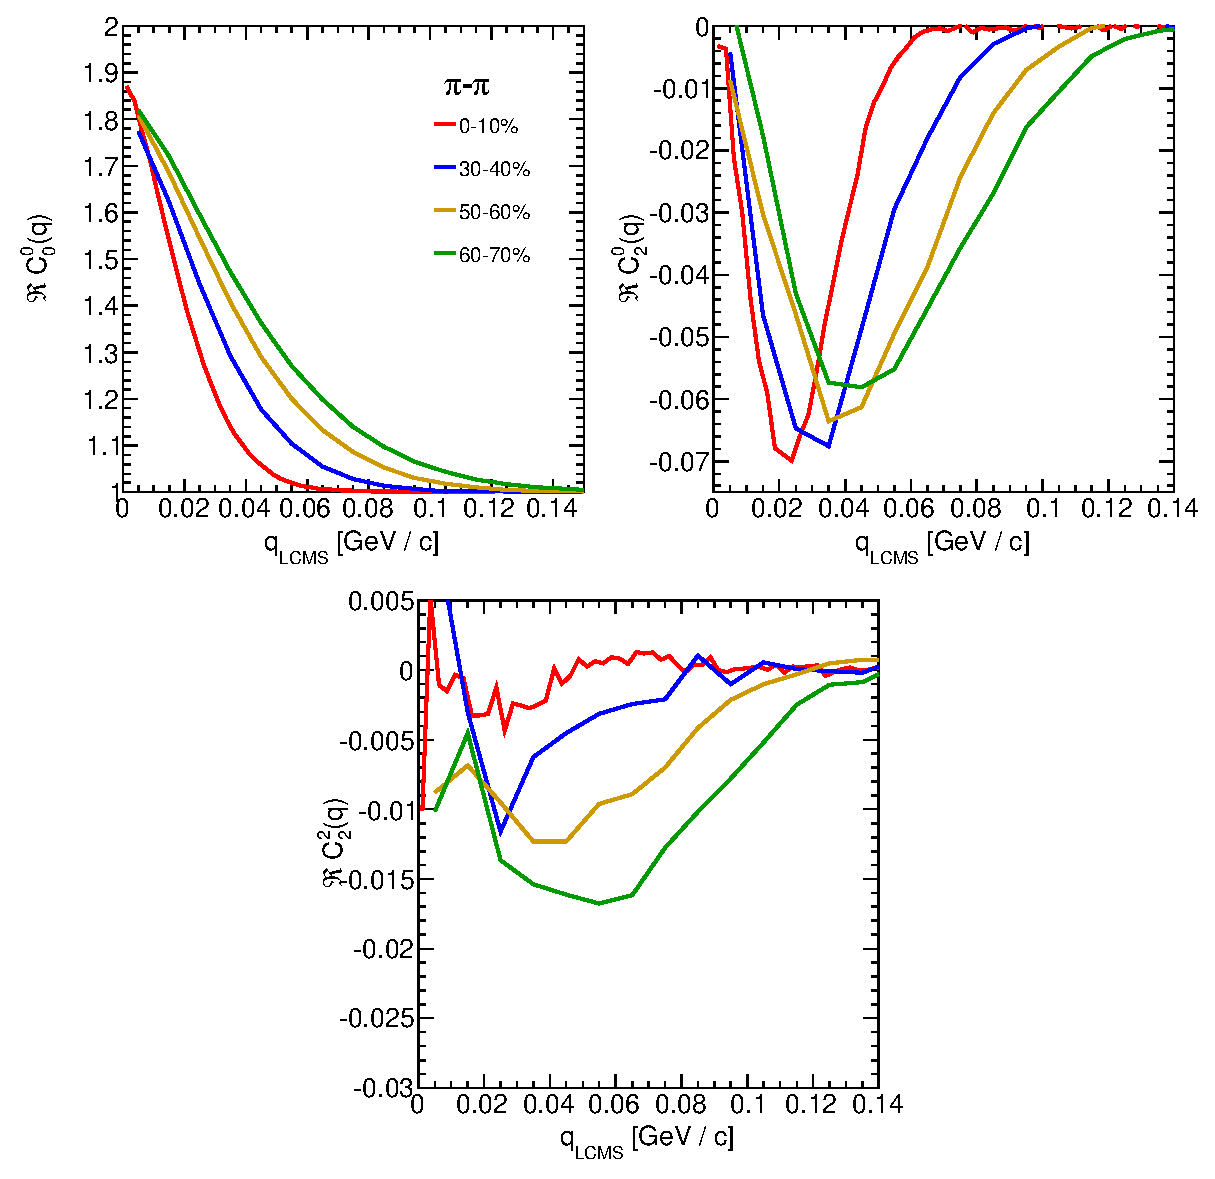
\includegraphics[width=1.0\textwidth]{results/cf3dpi}}
        \caption{Spherical harmonics coefficients of the two-pion correlation function. From the top left: $\Re C^0_0$, $\Re C^0_2$ and $\Re C^2_2$. Only few centrality bins are presented for increased readability.}
      \label{fig:cf3dpi}
      \end{figure}

      \begin{figure}[b]
        \centering
        \centerline{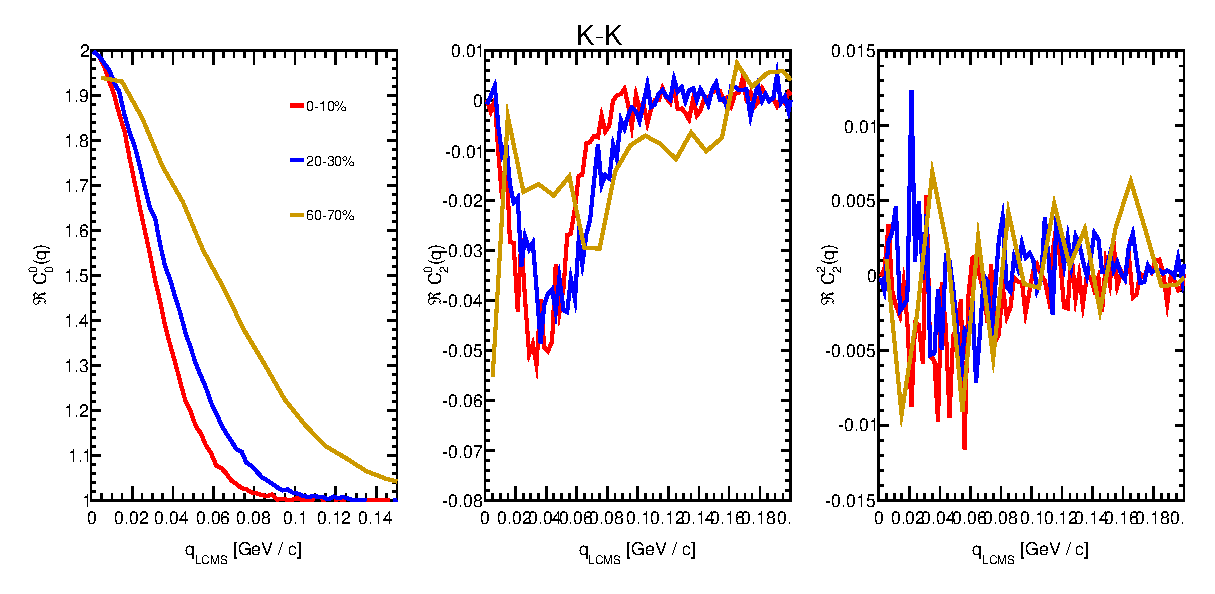
\includegraphics[width=1.0\textwidth]{results/cf3dk}}
        \caption{Spherical harmonics coefficients of the two-kaon correlation function. From the top left: $\Re C^0_0$, $\Re C^0_2$ and $\Re C^2_2$. Only few centrality bins are presented for increased readability. The $\Re C^2_2$ is noisy, but one can still notice that it differs from zero and is becoming negative.}
      \label{fig:cf3dk}
      \end{figure} 

      \begin{figure}[b]
        \centering
        \centerline{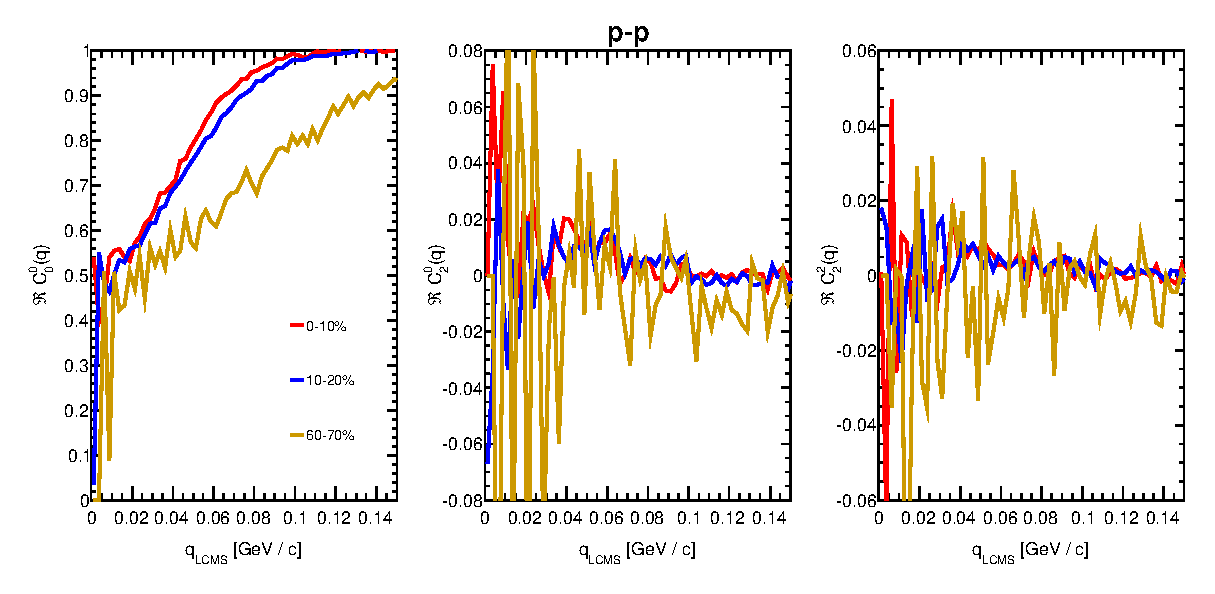
\includegraphics[width=1.0\textwidth]{results/cf3dp}}
        \caption{Spherical harmonics coefficients of the two-proton correlation function. From the top left: $\Re C^0_0$, $\Re C^0_2$ and $\Re C^2_2$. Only few centrality bins are presented for increased readability. The $\Re C^0_2$ and $\Re C^2_2$ are noisy, but one can still notice, that they differ from zero and are becoming positive.}
      \label{fig:cf3dp}
      \end{figure}

      The three-dimensional correlation functions as functions of relative momentum $q_{LCMS}$ were calculated in a form of spherical harmonics components series accordingly to the Eq.~\ref{eq:sh_decomposition}.
      In the femtoscopic analysis of identical particles, the most important information is stored in the $\Re C^0_0$, $\Re C^0_2$ and $\Re C^2_2$.
      Correlation functions obtained in this procedure for different centrality bins for the pairs of pions, kaons and protons are presented in the Fig.~\ref{fig:cf3dpi}, \ref{fig:cf3dk} and \ref{fig:cf3dp}.
      
      Coefficients for pairs of identical bosons (pions and kaons) are shown in the Fig.~\ref{fig:cf3dpi} and \ref{fig:cf3dk}.
      The increase of a correlation in the low momenta regime is clearly visible in the $\Re C^0_0$ component and has its source in the Bose-Einstein statistics.
      The $\Re C_0^0$ resembles one-dimensional correlation function and in fact it encodes information about overall source radius.
      The second coefficient $\Re C^0_2$ differs from zero (is negative), which yields the information about the ratio $R_T / R_{long}$.
      The $\Re C^2_2$ stores the $R_{out} / R_{side}$ ratio and one can notice that is non-vanishing (is also negative).

      The correlation function for a pair of identical fermions is in the Fig.~\ref{fig:cf3dp}.
      An influence of Fermi-Dirac statistics has its effect in the decrease of a correlation down to 0.5 at low relative momentum, which can be observed in $\Re C^0_0$.
      The $\Re C^0_2$ and $\Re C^2_2$ coefficients differ from zero and become positive.

      The common effect for the spherical harmonics form of a correlation function is the ``mirroring'' of the shape of the $\Re C^0_0$ coefficient - when correlation function decreases, the $\Re C^0_2$ and $\Re C^2_2$ are becoming positive and vice versa.
      This is quite different behaviour than in the case of correlations of non-identical particles, where the $\Re C^0_2$ still behaves in the same manner, but $\Re C_2^2$ has the opposite sign to the $\Re C^0_2$~\cite{nonidfemto}.

      In all cases, the correlation function gets wider with the peripherality of a collision i.e. the correlation function for most central collisions (0-10\%) is much narrower than for the most peripheral ones (60-70\%).
      This phenomena in clearly visible the $\Re C^0_0$ coefficients.
      Other components are also affected by this effect, this is especially noticeable in the case of kaons and pions.
      For the protons, the results are noisy, hence this effect is not distinguishable.

      % The quantitative analysis of the trends in the shape (described by the femtoscopic radii) of a three-dimensional correlation function is performed in the next section of this chapter.

    \FloatBarrier
    \clearpage
    %
    % ========
    \subsection{Centrality dependence of a correlation function}
    % ========
      The centrality dependence of a correlation function is especially visible in one-dimensional correlation functions.
      This effect is presented in the Fig.~\ref{fig:centr_dep} - the width is smaller in the most central collisions.
      Hence, the femtoscopic radii (proportional to the inverse of width) is increasing with the centrality.
      An explanation for this growth is that in the most central collisions, a size of a created system is larger than for the peripheral ones.
      \begin{figure}[h]
        \centering
        \centerline{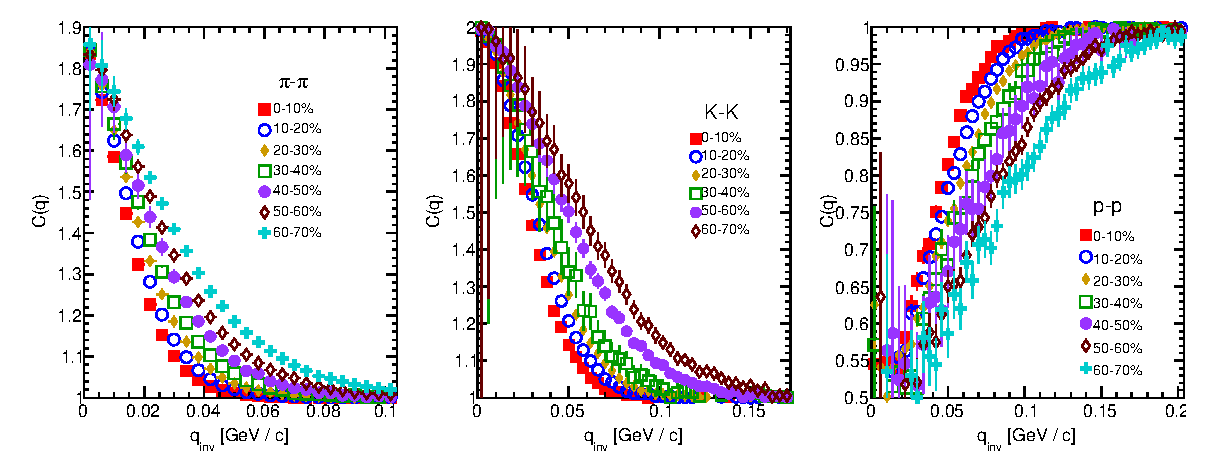
\includegraphics[width=1.0\textwidth]{results/cfvsctr}}
        \caption{One-dimensional correlation function for pions, kaons and protons for different centralities.}
      \label{fig:centr_dep}
      \end{figure}
    \FloatBarrier
    \clearpage
    %
    % ========
    \subsection{$k_T$ dependence of a correlation function}
    % ========
      In the Fig.~\ref{fig:kt_dep} there are presented one-dimensional correlation functions for pions, kaons and protons for the same centrality bin, but different $k_T$ ranges.
      One can observe in all cases of the particle types, appearance of the same trend: with the increase of the total transverse momentum of a pair, the width of a correlation function increases and the femtoscopic radius decreases.
      The plots in the Fig.~\ref{fig:kt_dep} were zoomed in to show the influence of $k_T$.

      \begin{figure}[h]
        \centering
        \centerline{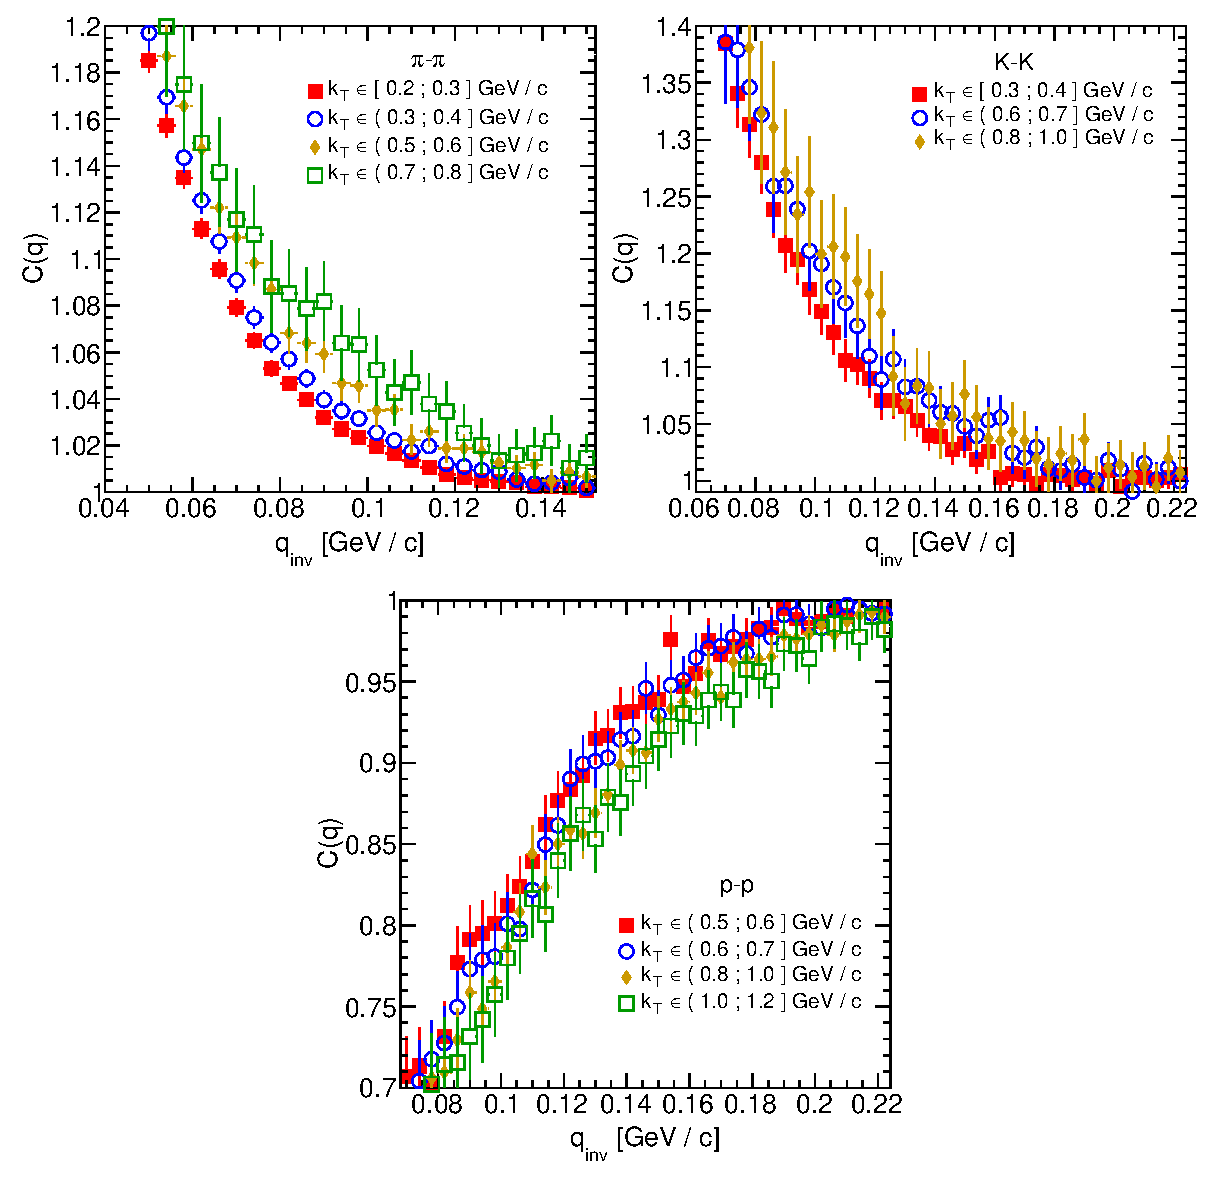
\includegraphics[width=1.0\textwidth]{results/cfvskt}}
        \caption{One-dimensional correlation functions for pions, kaons and protons, for the same centrality bin and different $k_T$ ranges. The plot was zoomed in to the region which illustrates the $k_T$ dependence in the best way. Only few of the calculated ranges are presented for better readability.}
      \label{fig:kt_dep}
      \end{figure}
    \FloatBarrier
    \clearpage
  %
  % ========
  \section{Results of the fitting procedure}
  % ========
  In order to perform a quantitative analysis of a wide range of correlation functions, the theoretical formulas were fitted to the calculated experimental-like data.
  In this procedure, the femtoscopic radii for the three-dimensional as well as one-dimensional correlation functions were extracted.
  The main goal of this analysis is a verification of a transverse mass scaling of different particles types.
  The radii are plotted as a function of a transverse mass $m_T = \sqrt{k_T^2 +m^2}$ and the following power-law is fitted:
  \begin{equation}
    \label{eq:power-law}
    R_x = \alpha {m_T}^{-\beta}~,
  \end{equation}
  where the $\alpha$ and $\beta$ are free parameters.
    %
    % ========
    \subsection{The three-dimensional femtoscopic radii scaling}
    % ========
      \begin{figure}[b]
        \centering
        \centerline{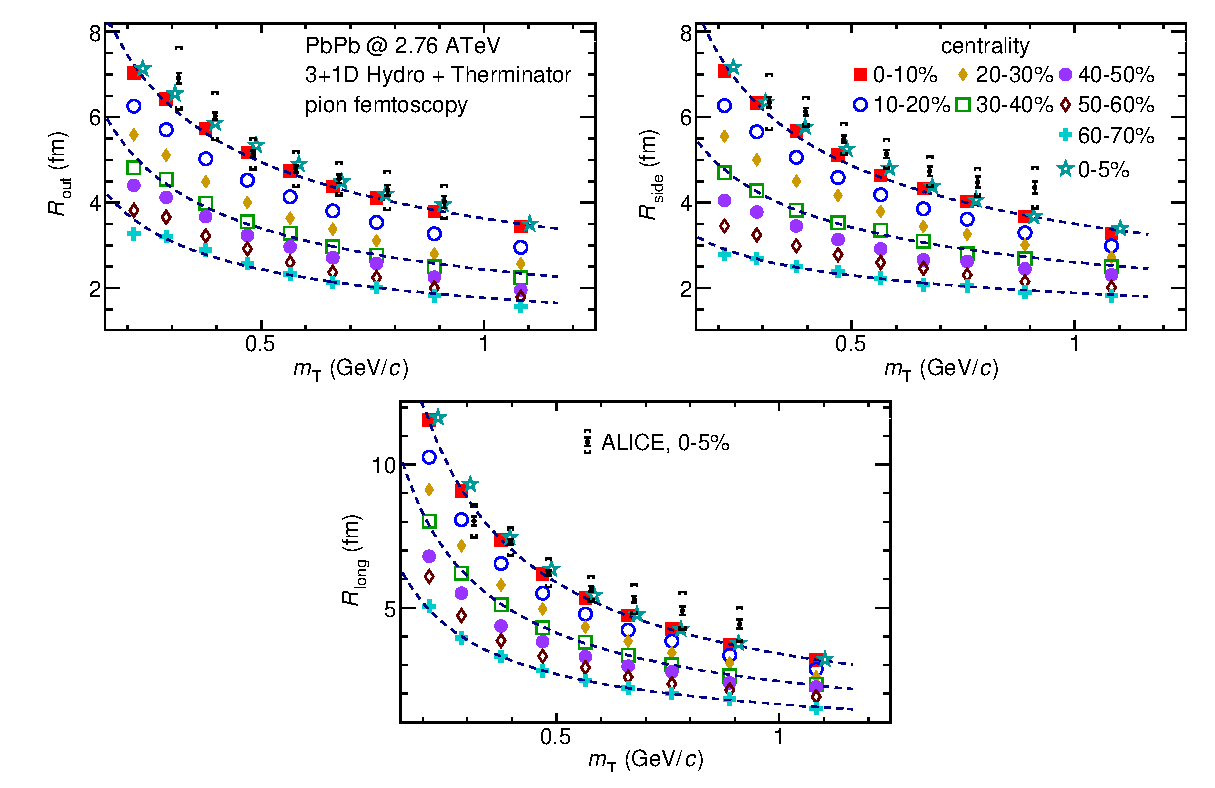
\includegraphics[width=1.05\textwidth]{results/piradii}}
        \caption{Femtoscopic radii in LCMS coming from two-pion correlation functions for all centrality bins as a function of $m_T$. The dashed lines are power-law fits. The most central collisions (0-5\%) are compared to the results from ALICE~\cite{alice_pion}. The two datasets are shifted to the right for visibility~\cite{galazyn}.}
        \label{fig:piradii}
      \end{figure}

      In the Fig.~\ref{fig:piradii} there are femtoscopic radii in the outward, sideward and longitudinal direction of the analysis of two-pion correlation functions in LCMS.
      The dashed lines are fits of the power law to the data.
      One can notice, that the power law describes well data points with a 5\% accuracy.
      The $\beta$ parameter for the outward direction is in the order of 0.45.
      For the sideward direction, this parameter has the similar value, but it is lower for the most peripheral collisions.
      In case of the longitudinal direction, the $\beta$ has greater value, up to 0.75.
      A larger value in case of longitudinal direction is an indication of a strong transverse expansion of created system.
      In the Fig.~\ref{fig:piradii} there are also compared results for the top 5\% central collisions (star-shaped markers) with experimental data from ALICE~\cite{alice_pion}.
      The experimental results are consistent with the ones coming from the model predictions.
      % \begin{figure}[b]
      %   \centering
      %   \centerline{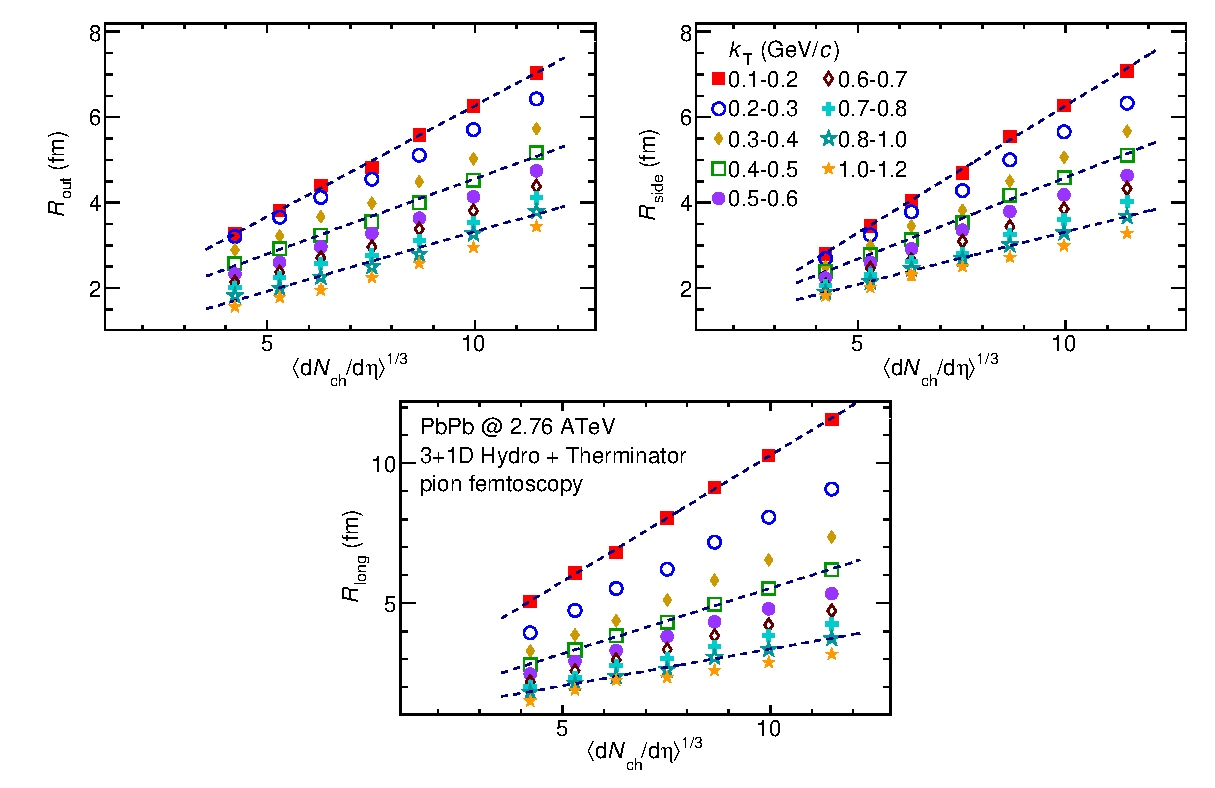
\includegraphics[width=1.05\textwidth]{results/piradii_vs_nch}}
      %   \caption{no caption~\cite{galazyn}.}
      % \label{fig:piradii}
      % \end{figure}   
      \begin{figure}[b]
        \centering
        \centerline{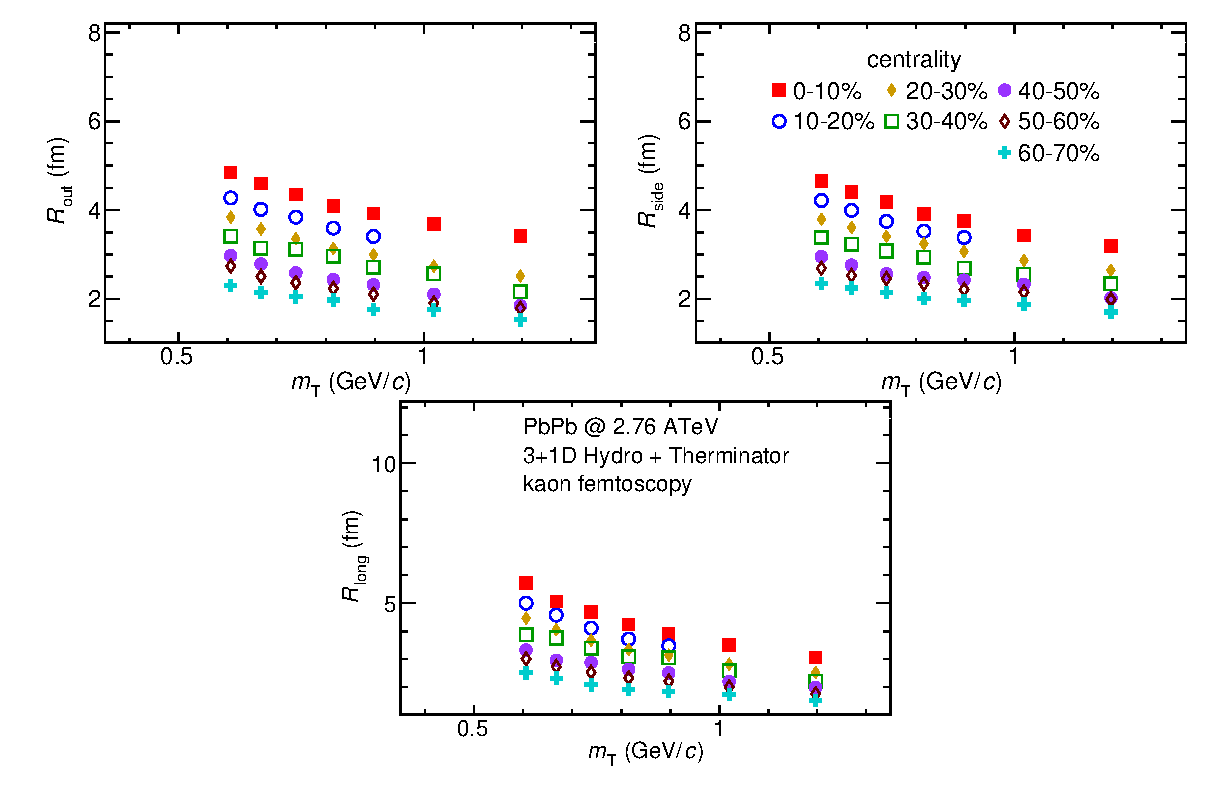
\includegraphics[width=1.05\textwidth]{results/kradii}}
        \caption{Femtoscopic radii extracted from two-kaon correlation functions for different centrality bins as a function of $m_T$.~\cite{galazyn}.}
      \label{fig:kradii}
      \end{figure}

      The Fig.~\ref{fig:kradii} presents femtoscopic radii coming from the kaon calculations.
      The $R_{out}$, $R_{side}$ and $R_{long}$ fall also with the power-law within the 5\% accuracy.
      The $\beta$ parameter was larger in case of kaons: 0.59 in outward direction, 0.54 in the sideward and 0.86 for longitudinal.

      The results for two-proton analysis are shown in the Fig.~\ref{fig:pradii}.
      The Eq.~\ref{eq:power-law} was fitted to the data and tells that the protons also follow the $m_T$ scaling within 5\% range.
      The $\beta$ parameter values were even bigger for the outward ( 0.58 ), sideward ( 0.61 ) and longitudinal ( 1.09 ) directions than for the other particle types. 

      \begin{figure}[b]
        \centering
        \centerline{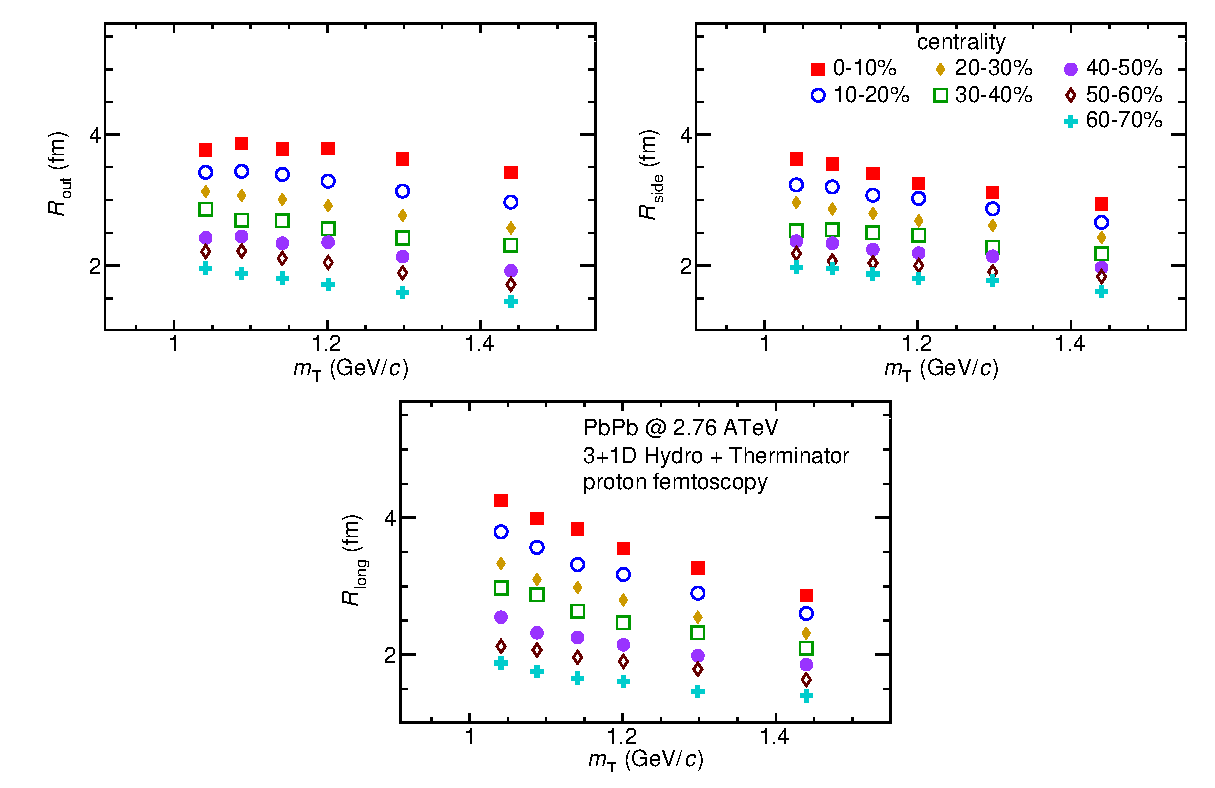
\includegraphics[width=1.05\textwidth]{results/pradii}}
        \caption{Femtoscopic radii extracted from two-proton correlation functions for different centrality bins as a function of $m_T$.~\cite{galazyn}.}
      \label{fig:pradii}
      \end{figure}

      \begin{figure}[b]
        \centering
        \centerline{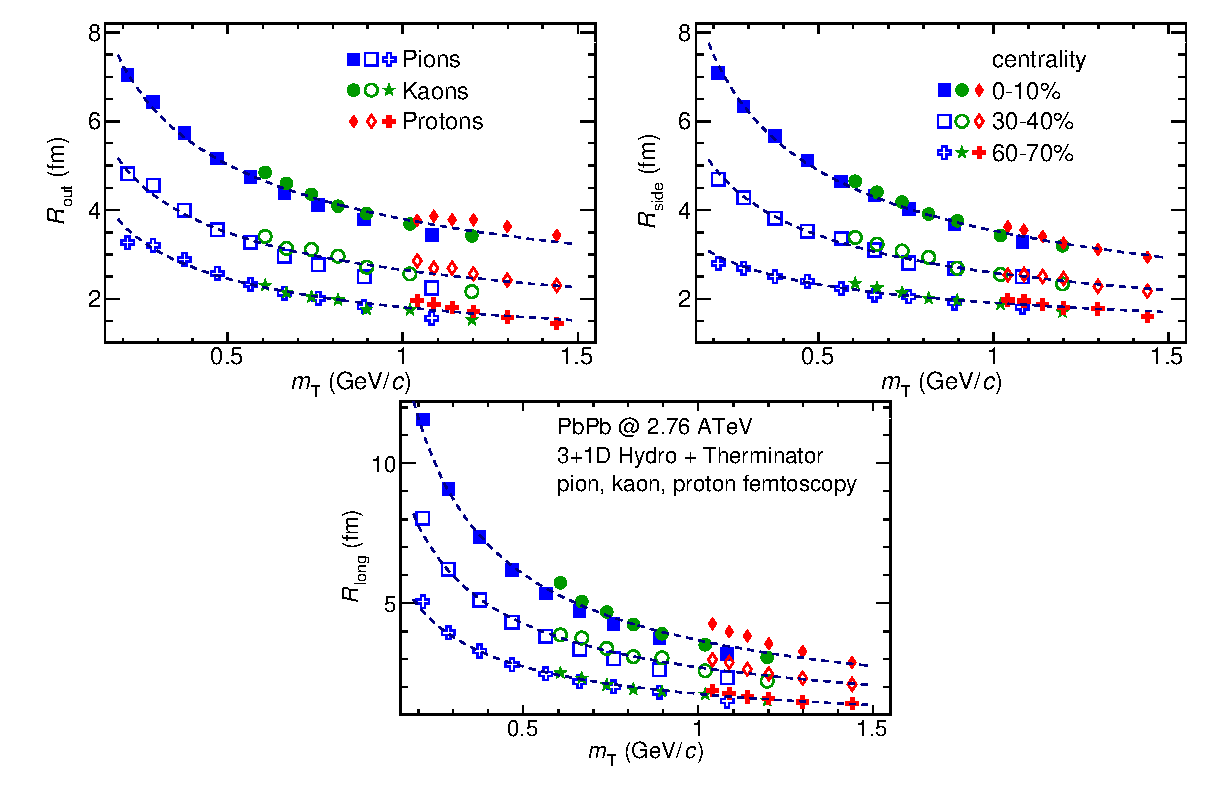
\includegraphics[width=1.05\textwidth]{results/allradii_lcms}}
        \caption{The results from the calculations for the pions, kaons and protons in for the three centralities presented on the common plot. One can notice that radii for particular centralities and different particle types follow the common power-law scaling.~\cite{galazyn}.}
      \label{fig:allradii}
      \end{figure}    

      The Fig.~\ref{fig:allradii} presents results for the pions, kaons and protons as a function of $m_T$.
      Considering differences in the $\beta$ value for the fits for different particles, one can suspect that there is no common scaling between different kinds of particles.
      However, when all of the results shown on the same plot, they are aligning on the common curve and the scaling is well preserved.
      The scaling accuracy is 3\%, 5\% and 4\% for the 0-10\%, 20-30\% and 60-70\% for the outward direction.
      For the sideward radii the scaling is better, with the average deviations 2\%, 2\% and 3\% respectively.
      In case of longitudinal direction the accuracy is 6\%, 5\% and 3\% for the three centralities.
      The $\beta$ parameter for the outward direction is close to the 0.42 in all cases.
      For the sideward direction it varies from 0.28 to 0.47 and is bigger for more central collisions.
      Regarding longitudinal radii, the exponent is bigger than the other two: $\beta \in [0.62 ; 0.72]$~.
      Considering all results, the plotted radii are following the common power-law scaling within the 5\% accuracy for all directions, centralities and particle types.
      \FloatBarrier
      %
      % ========
      \subsection{Scaling of one-dimensional radii}
      % ========
      \begin{figure}[b]
        \centering
        \centerline{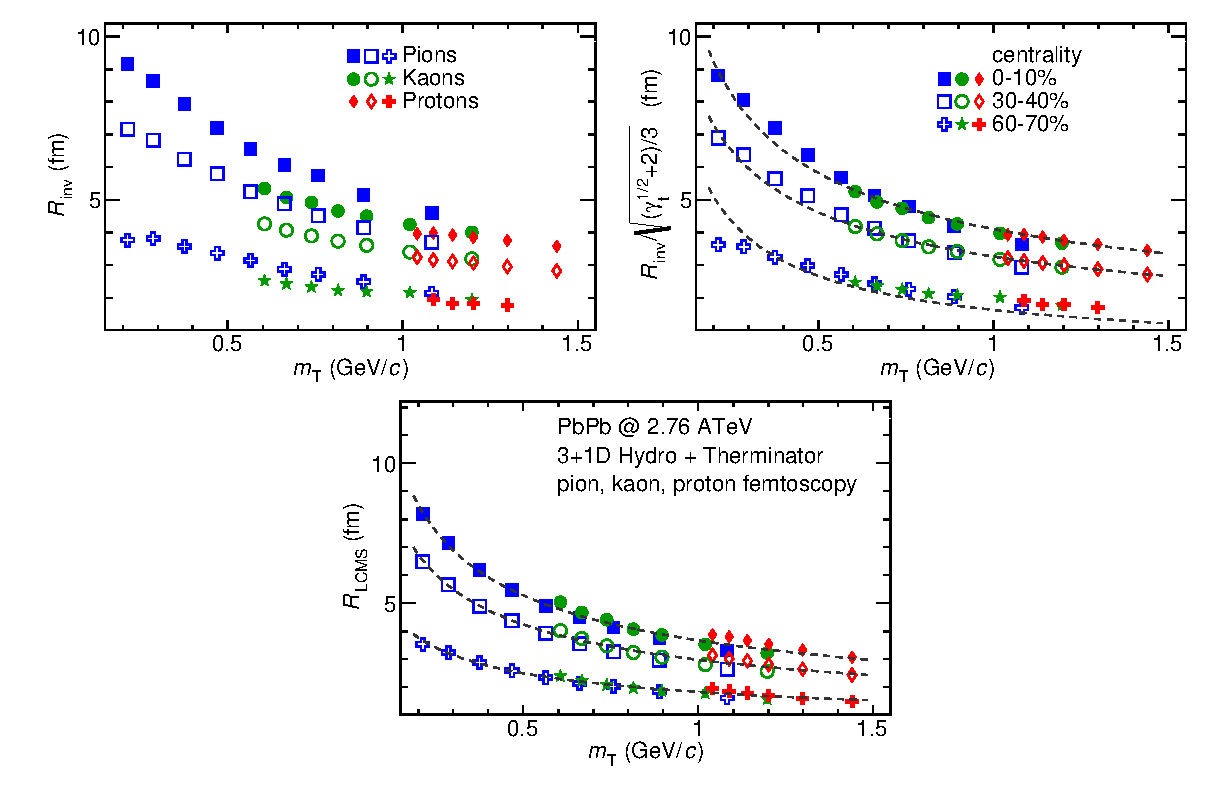
\includegraphics[width=1.05\textwidth]{results/scaling_test}}
        \caption{no caption~\cite{galazyn}.}
      \label{fig:scaling_test}
      \end{figure}    

      \begin{figure}[b]
        \centering
        \centerline{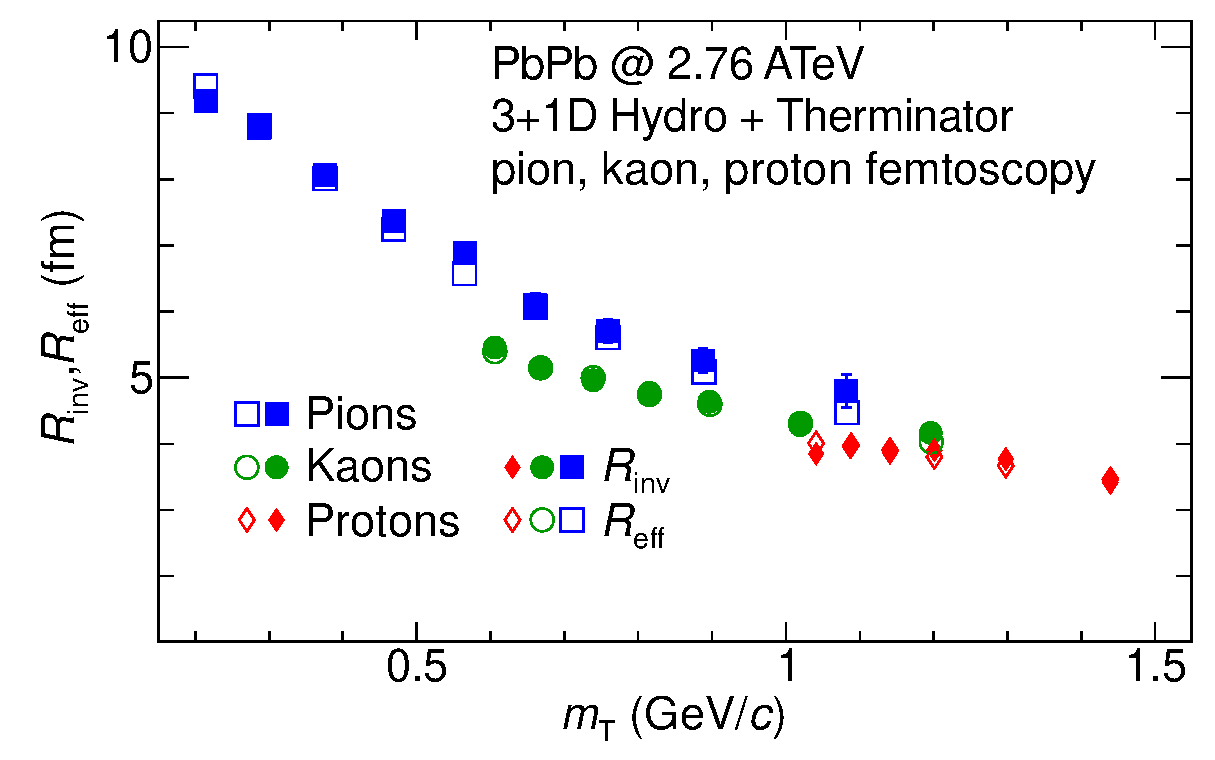
\includegraphics[width=0.55\textwidth]{results/rinvreff}}
        \caption{no caption~\cite{galazyn}.}
      \label{fig:rinveff}
      \end{figure}


      \FloatBarrier
  %
  % ========
  \section{Discussion of results}
  % ========

  %% nawiazanie do pracy sinyukova, karpenki,  o złamanym skalowaniu mt w przypadku rescatteringu
